%%%%%%%%%%%%
%
% $Autor: Chantal Crety $
% $Datum: 11.07.2025 $
% $Pfad: DemonstratorSchrittmotor\DemontageAnleitung\Demontage.tex
% $Beschreibung: Hauptteil der DemontageAnleitung
%
%%%%%%%%%%%%

\chapter {Demontage Geschwindigkeitssensor}

\section{Geschwindigkeitssensor Teil 1}
Lösen Sie die Mutter des Geschwindigkeitssensors auf der Armunterseite des rechten Gehäusekörpers. Verschieben Sie den Sensor entlang der vorgesehenen Nut um etwa 20 mm in Richtung Frontseite, bis zur nächsten Markierung – vorausgesetzt, Sie verwenden das Originalgehäuse.
Sollten bauliche Änderungen am Gehäuse vorgenommen worden sein, positionieren Sie den Sensor so weit wie möglich von seiner ursprünglichen Einbaulage entfernt nach vorn.
Diese Maßnahme gewährleistet ausreichenden Freiraum für die Lochscheibe bei der anschließenden Entfernung des Gehäuses. Ziehen Sie die Mutter nach dem Justieren wieder sorgfältig fest, um sie in der neuen Position zu fixieren.


\chapter{Entfernung der Gehäusehälften}

Die Entfernung der Gehäusekörper wird im Folgenden anhand der linken Hälfte beschrieben. Die Schritte lassen sich in gleicher Weise auf die rechte Gehäusehälfte übertragen.

Für die Demontage benötigen Sie beide Hände. Positionieren Sie sich frontal zur Blende und greifen Sie mit einer Hand an die Unterseite des linken Gehäuses – an jene Stelle, an der im Betriebszustand das Netzkabel austritt. 
Greifen Sie mit einer Hand an die Unterseite des linken Gehäuses, an die Stelle, an der sich im Betriebszustand das Netzkabel befindet. An dieser Position befindet sich eine größere Aussparung (siehe Abb.5.1), die sowohl bei der Montage als auch bei der Demontage genutzt wird.

Greifen Sie mit Ihren Fingern in die Öffnung und drücken Sie vorsichtig den unteren Teil des Gehäuses mitsamt der Halterungen aus der unteren Profilnut. Sobald dies erfolgt ist, können Sie das Gehäuse leicht bewegen. Üben Sie anschließend sanften Zug an der oberen Halterung aus und spreizen Sie das Gehäuse so weit auf, dass es sich aus der oberen Nut zu Ihnen hin herausziehen lässt.

Verharren Sie mit den Haltern zunächst auf den Profilen und ziehen Sie das Gehäuse nicht direkt gerade zu sich. Sie werden durch die Endschalterhalterung auf wiederstandtreffen.


\vspace{0.5cm}.
\begin{figure}[H]
	\centering
	\begin{minipage}{0.32\linewidth}
		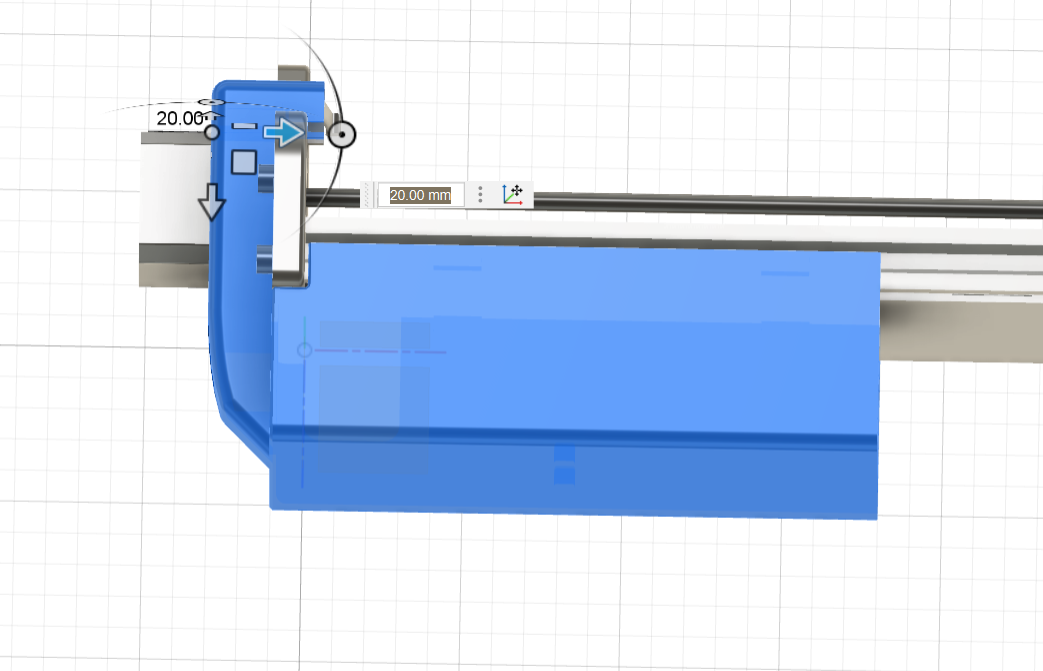
\includegraphics[width=\linewidth]{Images/Positionierung5.2.png}
		\caption*{Bild 1: Ursprungsposition}
	\end{minipage}
	\hfill
	\begin{minipage}{0.32\linewidth}
		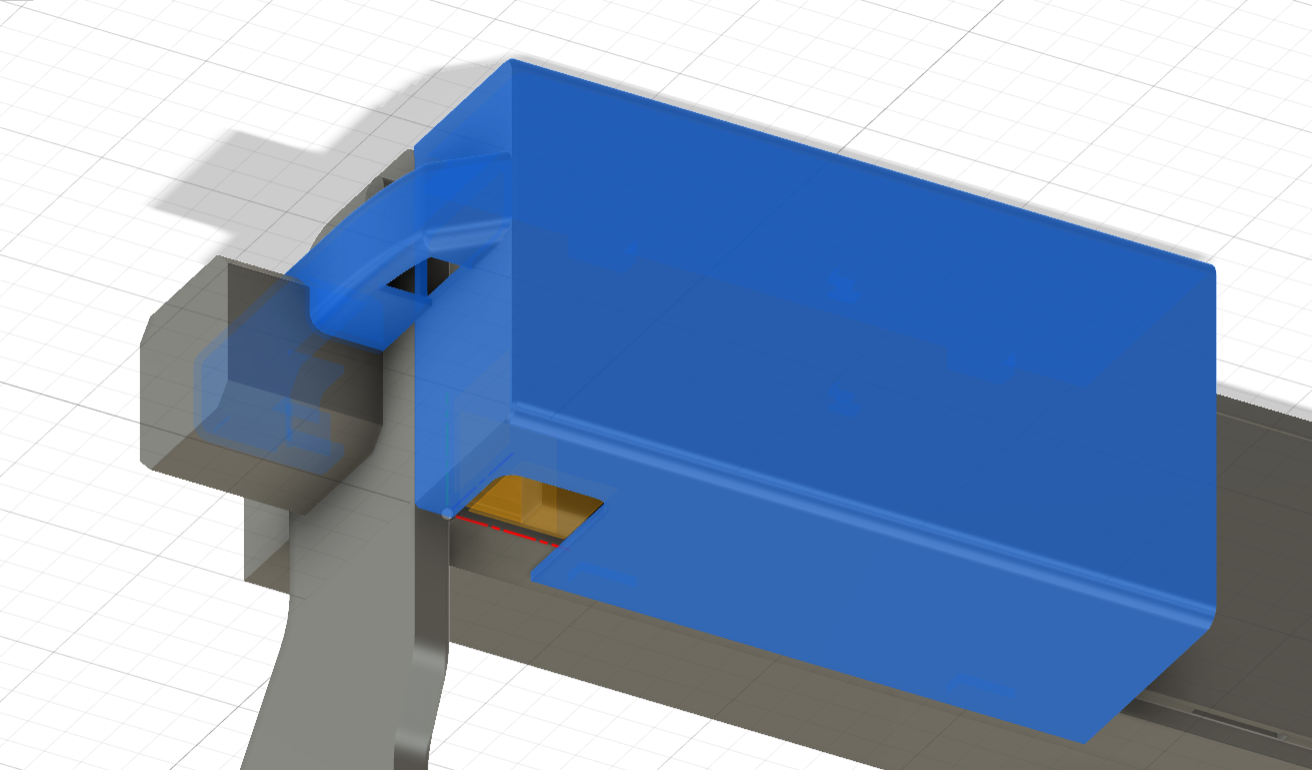
\includegraphics[width=\linewidth]{Images/Positionierung0.png}
		\caption*{Bild 2: Auslassung}
	\end{minipage}
	\hfill
	\begin{minipage}{0.32\linewidth}
		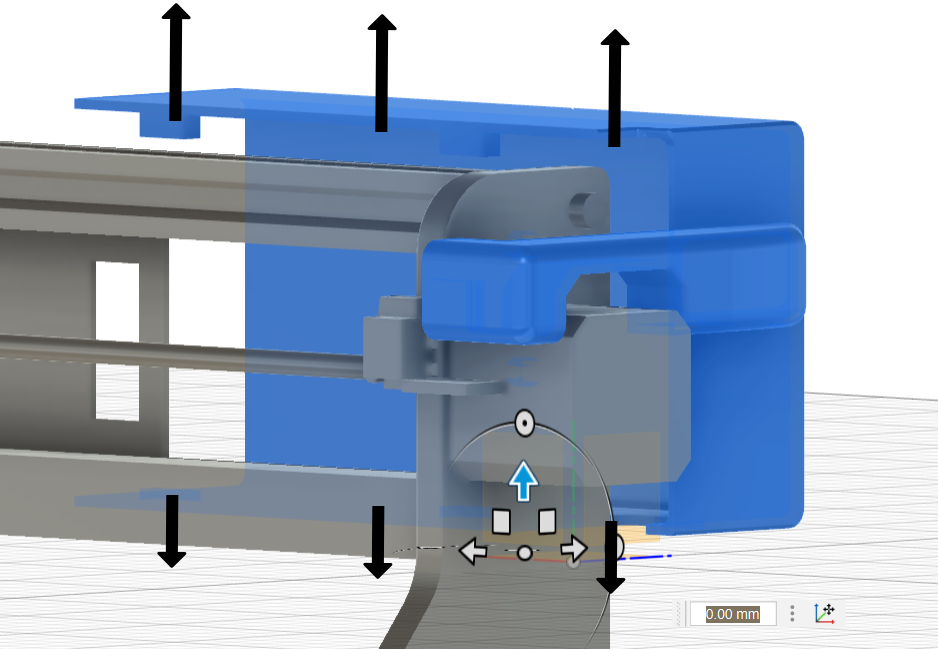
\includegraphics[width=\linewidth]{Images/Positionierung3.png}
		\caption*{Bild 2: Druckrichtungen}
	\end{minipage}
	\caption{Positionierungen zur Einhängung 1}
	\label{fig:positionierung_gehaeuse1}
\end{figure}
\vspace{0.5cm}
Nun kann das Gehäuse entlang der Profilführung vorsichtig nach links geschoben werden, bis es durch die Aussparung an einen Widerstand stößt (siehe Abb. 5.2).
\vspace{0.5cm}
\begin{figure}[H]
	\centering
	\begin{minipage}{0.48\linewidth}
		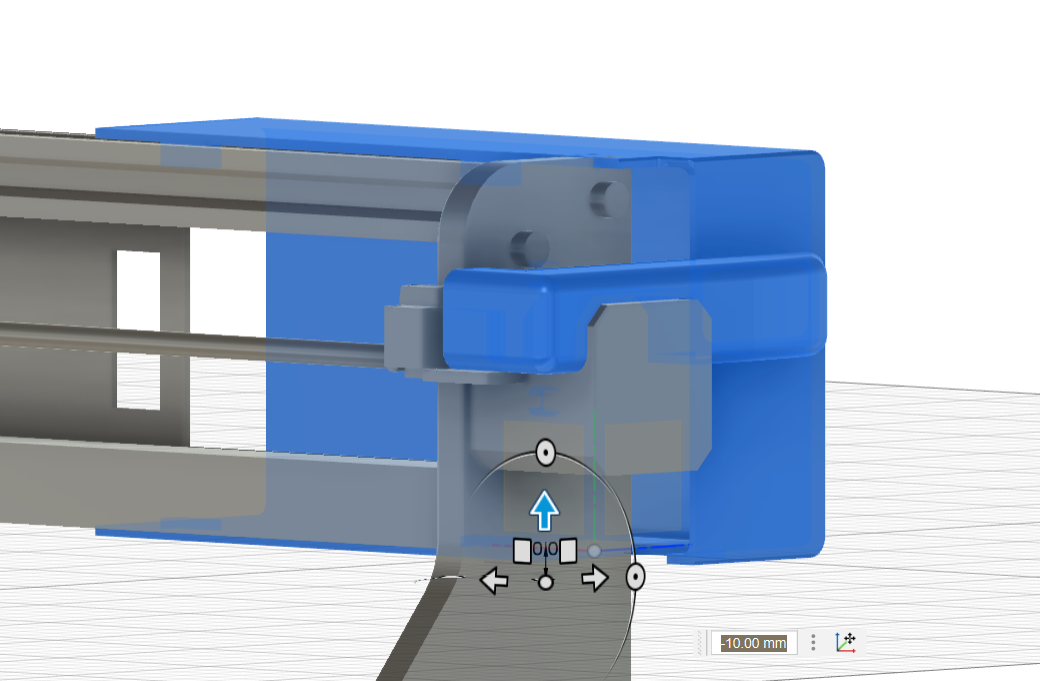
\includegraphics[width=\linewidth]{Images/Positionierung4.png}
		\caption*{Bild 1: Halt auf dem Profil}
	\end{minipage}
	\hfill
	\begin{minipage}{0.48\linewidth}
		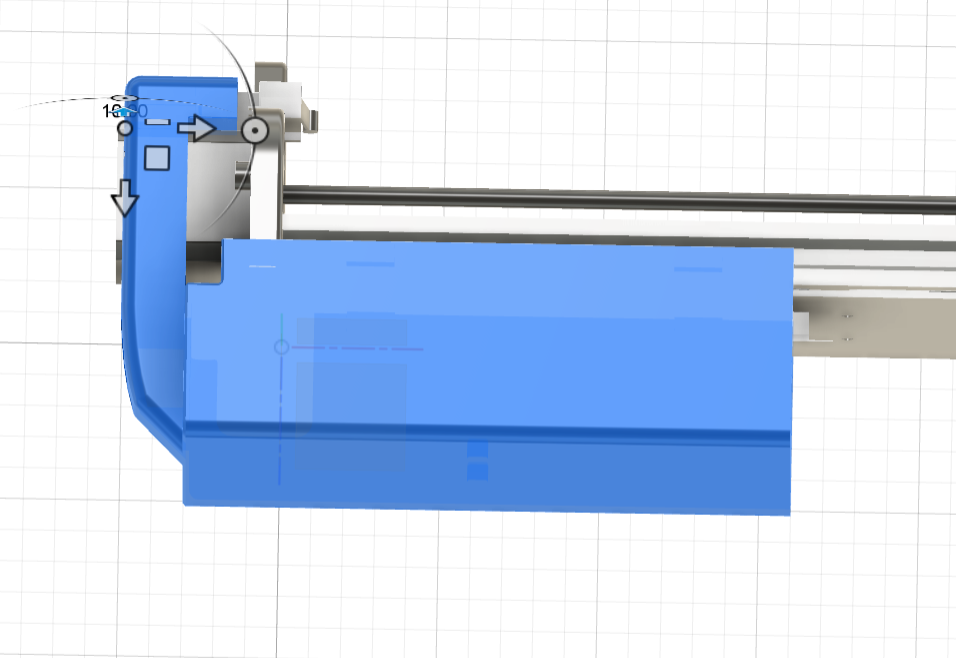
\includegraphics[width=\linewidth]{Images/Positionierung5.png}
		\caption*{Bild 2:Abschieben}
	\end{minipage}
	\caption{Positionierung bei der Aushängung 2}
	\label{fig:positionierung_gehaeuse2}
\end{figure}

In dieser Position lässt sich der Gehäusekörper abschließend vollständig nach oben abnehmen.

\vspace{0.5cm}
\begin{figure}[H]
	\centering
	\begin{minipage}{0.48\linewidth}
		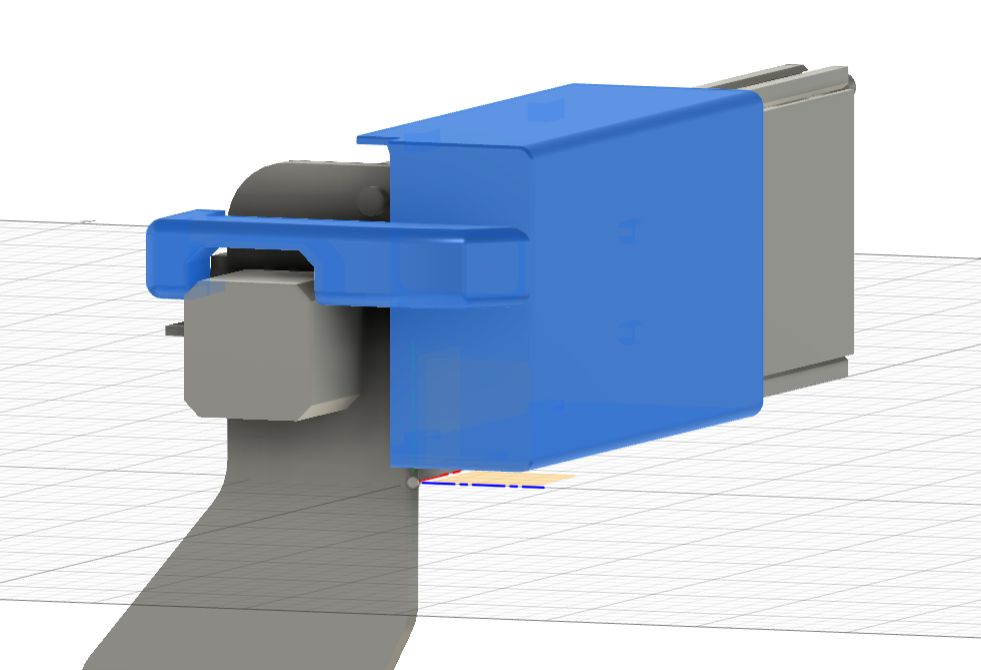
\includegraphics[width=\linewidth]{Images/Positionierung2.png}
		\caption*{Bild 1: Abnahme}
	\end{minipage}
	\hfill
	\begin{minipage}{0.48\linewidth}
		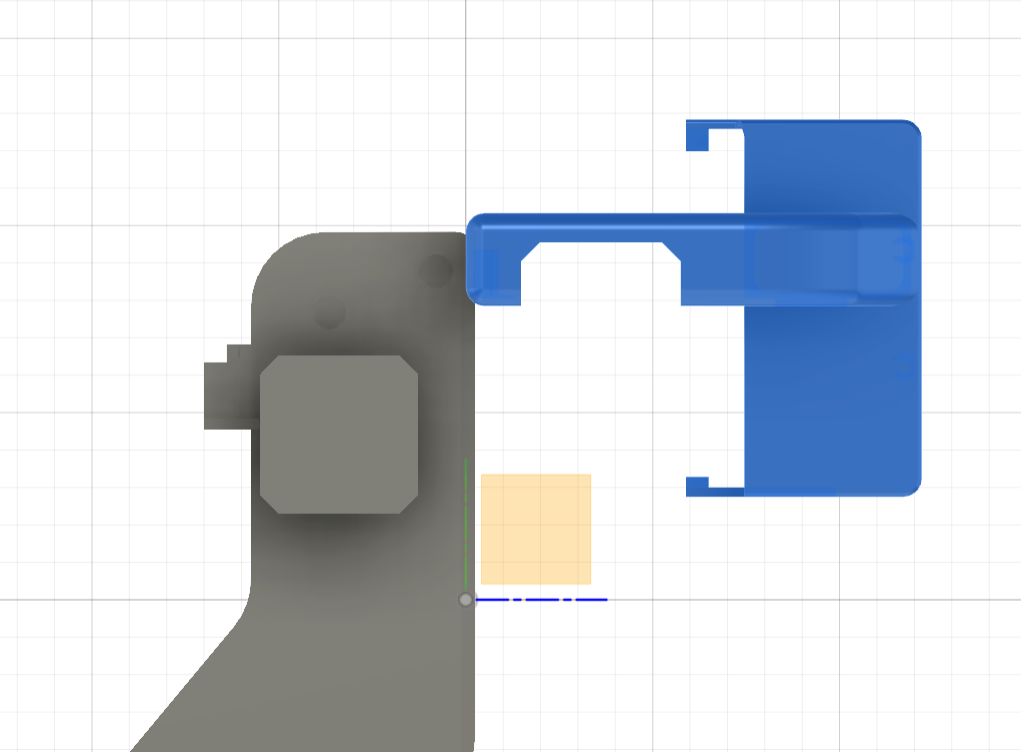
\includegraphics[width=\linewidth]{Images/Positionierung1.2.png}
		\caption*{Bild 2: Abnahme }
	\end{minipage}
	\caption{Positionierungen zur Aushängung 3}
	\label{fig:positionierung_gehaeuse3}
\end{figure}
\vspace{0.5cm}

Wiederholen Sie den Prozess für die rechte Seite und achten Sie darauf, dass kein starker Zug auf die Kabel ausgeübt wird.

\chapter {Trennung der Elektronik vom Gehäuse}

\section{Geschwindigkeitssensor – Teil 2}
Lösen Sie erneut die Mutter des Geschwindigkeitssensors an der Unterseite des rechten Gehäusearms und entfernen Sie sowohl die Mutter als auch die zugehörige Unterlegscheibe. Anschließend können die Kabel abgezogen und die Sensorhalterung zur Seite gelegt werden.
Lösen Sie danach die Mutter der Zylinderkopfschraube an der Spindelachse, welche sich am rechten Seitenträger des CNC-Tischs befindet. Dadurch lässt sich die Lochscheibe des Sensors von der verlängerten Achse abziehen. Bewahren Sie sämtliche Komponenten des Sensorsystems gemeinsam auf, um Verwechslungen zu vermeiden.

\section{Platten}
Die große und die kleine Montageplatte sind lediglich in den Profilnuten verklemmt und lassen sich von der Rückseite aus vorsichtig herausdrücken. Sollte sich eine Platte nur schwer lösen lassen, kann mit leichtem Zug von vorn nachgeholfen werden.

\subsection{Große Platte}
Das Steckbrett ist mit der Platte verklebt. Für die Demontage ist ein Cutter erforderlich. Gegebenenfalls kann ein geeignetes Lösemittel verwendet werden, um Kleberückstände zu entfernen.

\subsection{Kleine Platte}
Zur Entfernung des Entwicklerboards lösen Sie die beiden Senkkopfschrauben, indem Sie die Muttern auf der Rückseite der Platte entfernen.

\section{Display}
Das Display wird aus der Halterung gelöst, indem es zur Seite in Richtung der beiden Halteblöcke geschoben wird. Sobald sich die gegenüberliegende Seite unter dem einzelnen Halter freibewegt hat, kann das Display vorsichtig aus der Halterung herausgekippt oder -gedrückt werden.

\chapter{Trennen der Leitungen}
In diesem Schritt können sämtliche Steckverbindungen gelöst werden. Ziehen Sie dazu die Kabel vom Display, vom Arduino sowie vom Entwicklerboard vorsichtig ab. Achten Sie darauf, die Anschlüsse nicht zu beschädigen.

\section{Schalter}
Alle Schalter sind nun einseitig zugänglich und können vollständig demontiert werden. Je nach Schaltertyp besteht die restliche Befestigung entweder aus einer klemmenden Passform im Gehäuse oder einem aufgeschraubten Gewinde mit Kontermutter.

\subsection{Endschalter}

\begin{figure}[H]
	\vspace{1.5cm}
	\centering
	\tikzset{short/.style={}}
	\begin{tikzpicture}[scale=0.6, 
		every node/.style={font=\fontsize{800pt}{1000pt}\selectfont\bfseries}]
			\tikzstyle{every node}=[font=\LARGE]
			\draw [line width=1pt, short] (5.25,12) -- (5.25,9.75);
			\draw [line width=1pt, short] (5.25,9.75) -- (6.25,9.25);
			\draw [line width=1pt, short] (6,10) -- (5.75,10);
			\draw [line width=1pt, short] (5.75,10) -- (5.75,11.75);
			\draw [line width=1pt, short] (6,10) -- (6,11.75);
			\draw [line width=1pt, short] (6,11.25) -- (7.25,11);
			\draw [line width=1pt, short] (7.25,11) -- (7.75,11.25);
			\draw [line width=1pt, short] (7.75,12) -- (7.75,11.25);
			\draw [line width=1pt, short] (6.25,9.25) -- (6.25,6.75);
			\draw [line width=1pt, short] (9,11) -- (9,12.75);
			\draw [line width=1pt, short] (6.25,6.75) -- (3.75,8.5);
			\draw [line width=1pt, short] (3.75,8.5) -- (2,7.5);
			\draw [line width=1pt, short] (7.75,11.25) -- (6,11.5);
			\draw [line width=1pt, short] (6.5,11.75) -- (6.5,12.25);
			\draw [line width=1pt, short] (5.25,12) -- (6.5,11.75);
			\draw [line width=1pt, short] (6.5,11.75) -- (7.75,12);
			\draw [line width=1pt, short] (6.5,12.25) -- (9,12.75);
			\draw [line width=1pt, short] (6.5,12.25) -- (3.75,12.75);
			\draw [line width=1pt, short] (3.75,12.75) -- (0.25,12);
			\draw [line width=1pt, short] (9,12.75) -- (3.75,13.5);
			\draw [line width=1pt, short] (5.75,10) -- (5.25,10.25);
			\draw [line width=1pt, short] (3.75,12.75) -- (3.75,8.5);
			\draw [line width=1pt, short] (7,8.75) -- (9,7.5);
			\draw [line width=1pt, short] (9,7.5) -- (9,10.5);
			\draw [line width=1pt, short] (7,10.75) -- (7,8.75);
			\draw [line width=1pt, short] (7,10.75) -- (7.75,11);
			\draw [line width=1pt, short] (7.75,11) -- (9.5,10.75);
			\draw [line width=1pt, short] (9,10.5) -- (9.75,10.75);
			\draw [line width=1pt, short] (9.75,10.75) -- (9.75,8.25);
			\draw [line width=1pt, short] (9,7.5) -- (9.75,8.25);
			\draw [line width=1pt, short] (6.25,9.25) -- (7,9.5);
			\draw [line width=1pt, short] (7.25,11) -- (7.25,10.75);
			\draw [line width=1pt, short] (6,10) -- (7,9.5);
			\draw [line width=1pt, short] (6.25,6.75) -- (8.25,8);
			\draw [line width=1pt, short] (7,10.75) -- (9,10.5);
			\draw [line width=1pt, short] (7,10.25) -- (6.75,10.25);
			\draw [line width=1pt, short] (6.75,10.25) -- (6.75,10);
			\draw [line width=1pt, short] (6.75,10) -- (7,10);
			\draw [line width=1pt, short] (6.75,9.75) -- (6.75,9.5);
			\draw [line width=1pt, short] (6.75,9.75) -- (7,9.75);
			\draw [line width=1pt, short] (6.75,9.5) -- (7,9.5);
			\draw [line width=1pt, short] (7,9.25) -- (6.75,9.25);
			\draw [line width=1pt, short] (6.75,9.25) -- (6.75,9);
			\draw [line width=1pt, short] (6.75,9) -- (7,9);
			\draw [line width=1pt, short] (9.5,10.75) .. controls (10.5,9.75) and (10.75,9.5) .. (9.75,8.25);
			\draw [line width=1pt, short] (9.25,10.5) .. controls (10.5,9.75) and (10,9.25) .. (9.5,8.25);
			\draw [line width=1pt, dashed] (6.75,9.5) -- (5.25,10.5);
			\draw [line width=1pt, dashed] (6.75,10.25) -- (5.25,10.75);
			\draw [line width=1pt, ->, >=Stealth, dashed] (7.25,9.75) -- (8.75,9);
			\draw [ line width=1pt ] (9.5,8.25) circle (0.5cm);
	\end{tikzpicture}

\caption{Endschalterposition}
\label{tikz:Endschalter}
\end{figure}

Die Endschalter befinden sich in den Endhalterungen der Gehäusearme und sind lediglich klemmend im Gehäuse fixiert. Sie können vorsichtig und gerade aus ihrer Position gezogen werden. Dies ist in Abbildung \ref{Endschalter} dargestellt.

\subsection{Wippschalter}
Der Wippschalter kann von der Gehäuseinnenseite aus durch leichten Druck nach außen entfernt werden.

\subsection{Drucktaster grün und rot}
Die Drucktaster sind mithilfe eines Gewinderings an der Innenseite des Gehäuses befestigt. Zur Demontage muss der Ring abgeschraubt und über das Anschlusskabel abgezogen werden. Anschließend lassen sich die Taster nach vorn aus den Gehäusebohrungen herausnehmen. Schrauben Sie die Ringe direkt wieder auf die Taster, um sie nicht zu verlieren.

\subsection{Encoder}
Zur Entfernung des Encoders ziehen Sie zunächst die Abdeckkappe der Drehachse nach vorne ab. Darunter befinden sich eine Unterlegscheibe und eine Mutter, die den Encoder an der Gehäuseaußenseite fixieren. Entfernen Sie die Mutter und ziehen Sie den Encoder vorsichtig nach innen aus dem Gehäuse. Schrauben Sie danach die Mutter und Unterlegscheibe wieder auf die Drehachse und setzen Sie die Abdeckkappe erneut auf.

\section{Ablöten}
\textbf{Sicherheitshinweise zum Umgang mit dem Lötkolben}

Beim Arbeiten mit dem Lötkolben ist besondere Vorsicht geboten, da hohe Temperaturen zu Verletzungen oder Schäden an elektronischen Komponenten führen können. Beachten Sie daher folgende Sicherheitshinweise:

\begin{itemize}
	\item Verwenden Sie den Lötkolben ausschließlich auf einer hitzebeständigen Unterlage und in einem gut belüfteten, windstillen Arbeitsbereich.
	\item Halten Sie ausreichend Abstand zu brennbaren Materialien.
	\item Schalten Sie den Lötkolben nach Gebrauch sofort aus und lassen Sie ihn vollständig abkühlen, bevor Sie ihn weglegen oder verstauen.
	\item Achten Sie beim Ablöten darauf, benachbarte Bauteile nicht zu überhitzen oder die Leiterbahnen zu beschädigen.
	\item Lassen Sie den Lötkolben niemals unbeaufsichtigt in eingeschaltetem Zustand.
\end{itemize}


Durch vorsichtiges Ablöten können nun alle Schalter von ihren jeweiligen Kabelverbindungen getrennt werden. Vergessen sie abschließend nicht die Zylinderkopfschraube von der Spindel mit abzulösen.

\chapter{Organisation}

Trennen Sie nun die letzten verbleibenden Kabelverbindungen mithilfe eines Seitenschneiders.
Bewahren Sie sämtliche Bauteile trocken, staubfrei und möglichst luftdicht auf – idealerweise in antistatischen Beuteln oder Behältern.Für einen späteren Wiederaufbau steht Ihnen die zugehörige Montageanleitung unterstützend zur Verfügung.